\documentclass[12pt,reqno]{amsart}
\usepackage[top=2cm, left=2cm,right=2cm,bottom=2cm]{geometry}
\renewcommand{\baselinestretch}{1.2}
\usepackage{amsmath}
\usepackage{amssymb}
\usepackage{color,hyperref,enumerate,multicol}
\definecolor{darkblue}{rgb}{0.0,0.0,0.3}
\hypersetup{colorlinks,breaklinks,
            linkcolor=darkblue,urlcolor=darkblue,
            anchorcolor=darkblue,citecolor=darkblue}
            
\usepackage{algorithm}
\usepackage{algorithmic}
\pagestyle{empty}
\newcommand{\N}{\ensuremath{\mathbb{N}}}
\newcommand{\Z}{\ensuremath{\mathbb{Z}}}
\newcommand{\R}{\ensuremath{\mathbb{R}}}
\newcommand{\meet}{\ensuremath{\wedge}}
\newcommand{\Meet}{\ensuremath{\bigwedge}}
\newcommand{\join}{\ensuremath{\vee}}
\renewcommand{\emptyset}{\ensuremath{\varnothing}}
\renewcommand{\subset}{\ensuremath{\subsetneq}}
\newcommand{\boldemph}{\emph}
\newcommand{\lcm}{\operatorname{lcm}}

\newcommand{\probskip}{\vskip1cm}

\newcommand{\subject}{MATH}
\newcommand{\coursenumber}{3140}
\newcommand{\semester}{Fall 2018}

\begin{document}
\thispagestyle{empty}

\noindent \textbf{\subject \coursenumber}\\
{\bf Homework 7} 
\vskip1cm
\noindent {\bf Exercises:} 1, 2 (below) and Judson 19.3, 19.13, 19.19.\\
{\bf Due date:} Friday, 10/19

\bigskip

\begin{enumerate}[{\bf 1.}]

%% 1 %%%%%%%%%%%%%%%%%%%%%%%%%%%%%%%%%%%%%%%%%%%%%%%%
\item %1
Let $P$ with $\leq$ be a partially ordered set, let $S \subseteq P$ and let
$u\in P$.  We say that $u$ is an \emph{upper bound} for $S$ iff $s\leq u$ for
all $s \in S$.  We say $\ell$ is the \emph{least upper bound} of $S$ iff $\ell$
is an upper bound of $S$ and $\ell \leq u$ for every upper bound $u$ of $S$.
Prove that if $\ell$ is the least upper bound of the set $\{x, y\}$ and $m$ is
the least upper bound of the set $\{\ell, z\}$, then $m$ is the least upper
bound of the set $\{x, y, z\}$.

\textbf{Answer:} Let $S = \{x, y, z\}$. We want to show that $m$ is the least upper bound of $S$. 

First, we know that $\ell$ is the least upper bound of $\{x, y\}$. This means that $\ell$ is an upper bound of $\{x, y\}$ and $\ell \leq u$ for every upper bound $u$ of $\{x, y\}$. 

Since $m$ is the least upper bound of $\{\ell, z\}$, we know that $m$ is an upper bound of $\{\ell, z\}$ and $m \leq u$ for every upper bound $u$ of $\{\ell, z\}$. 

Now, let's consider the set $S = \{x, y, z\}$. We need to show that $m$ is an upper bound of $S$ and $m \leq u$ for every upper bound $u$ of $S$. 

Since $\ell$ is an upper bound of $\{x, y\}$, we know that $x \leq \ell$ and $y \leq \ell$. 

Since $m$ is an upper bound of $\{\ell, z\}$, we know that $\ell \leq m$ and $z \leq m$. 

Combining these inequalities, we have $x \leq \ell \leq m$ and $y \leq \ell \leq m$ and $z \leq m$. 

Therefore, $m$ is an upper bound of $S$. 

Now, let $u$ be an upper bound of $S$. This means that $x \leq u$, $y \leq u$, and $z \leq u$. 

Since $\ell$ is the least upper bound of $\{x, y\}$, we have $\ell \leq u$. 

Since $m$ is the least upper bound of $\{\ell, z\}$, we have $m \leq u$. 

Therefore, $m$ is the least upper bound of $S$. 

Hence, if $\ell$ is the least upper bound of $\{x, y\}$ and $m$ is the least upper bound of $\{\ell, z\}$, then $m$ is the least upper bound of $\{x, y, z\}$. 

\probskip

%% 2 %%%%%%%%%%%%%%%%%%%%%%%%%%%%%%%%%%%%%%%%%%%%%%%%
\item
Let $(P, \leq)$ be a partially ordered set with the property that every pair of
elements $x, y \in P$ has a greatest lower bound. For $x, y\in P$, define 
$x \cdot y = \operatorname{glb}(x,y)$. Prove that $(P, \cdot)$ is a semilattice.

\textbf{Answer:} To prove that $(P, \cdot)$ is a semilattice, we need to show that for any $x, y \in P$, the operation $\cdot$ is well-defined and satisfies the semilattice properties.

First, let's show that $\cdot$ is well-defined. 

For any $x, y \in P$, we define $x \cdot y = \operatorname{glb}(x,y)$. Since every pair of elements in $P$ has a greatest lower bound, we know that $\operatorname{glb}(x,y)$ exists and is unique. Therefore, the operation $\cdot$ is well-defined.

Next, let's show that $\cdot$ satisfies the semilattice properties. 

1. \textbf{Associativity:} For any $x, y, z \in P$, we have $(x \cdot y) \cdot z = \operatorname{glb}(\operatorname{glb}(x,y), z)$ and $x \cdot (y \cdot z) = \operatorname{glb}(x, \operatorname{glb}(y,z))$. Since the greatest lower bound operation is associative, we have $(x \cdot y) \cdot z = x \cdot (y \cdot z)$.

2. \textbf{Commutativity:} For any $x, y \in P$, we have $x \cdot y = \operatorname{glb}(x,y) = \operatorname{glb}(y,x) = y \cdot x$.

3. \textbf{Idempotence:} For any $x \in P$, we have $x \cdot x = \operatorname{glb}(x,x) = x$.

Therefore, $(P, \cdot)$ satisfies the semilattice properties.

Hence, $(P, \cdot)$ is a semilattice.

\probskip
 
%% 3 %%%%%%%%%%%%%%%%%%%%%%%%%%%%%%%%%%%%%%%%%%%%%%%%
\item[{\bf 19.3.}] 
Draw a diagram of the lattice of subgroups of ${\mathbb Z}_{12}$.

\textbf{Answer:} The lattice of subgroups of ${\mathbb Z}_{12}$ can be represented as follows:

\begin{center}
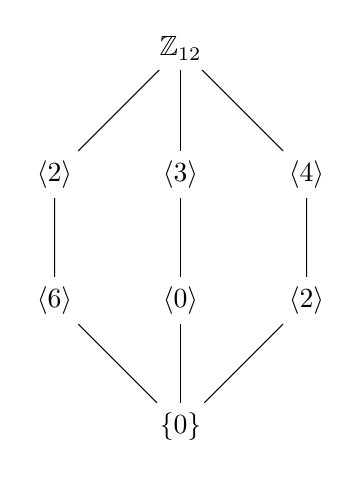
\begin{tikzpicture}[scale=0.8]
\node (G) at (0,0) {$\mathbb{Z}_{12}$};
\node (H1) at (-2,-2) {$\langle 2 \rangle$};
\node (H2) at (0,-2) {$\langle 3 \rangle$};
\node (H3) at (2,-2) {$\langle 4 \rangle$};
\node (H4) at (-2,-4) {$\langle 6 \rangle$};
\node (H5) at (0,-4) {$\langle 0 \rangle$};
\node (H6) at (2,-4) {$\langle 2 \rangle$};
\node (H7) at (0,-6) {$\{0\}$};

\draw (G) -- (H1);
\draw (G) -- (H2);
\draw (G) -- (H3);
\draw (H1) -- (H4);
\draw (H2) -- (H5);
\draw (H3) -- (H6);
\draw (H4) -- (H7);
\draw (H5) -- (H7);
\draw (H6) -- (H7);
\end{tikzpicture}
\end{center}

\probskip

%% 14 %%%%%%%%%%%%%%%%%%%%%%%%%%%%%%%%%%%%%%%%%%%%%%%%
\item[{\bf 19.13.}] 
Let $G$ be a group and $X$ be the set of subgroups of $G$ ordered by
set-theoretic inclusion. If $H$ and $K$ are subgroups of $G$, show
that the least upper bound of $H$ and $K$ is the subgroup generated by
$H \cup K$. 

\textbf{Answer:} Let $H$ and $K$ be subgroups of $G$. We want to show that the least upper bound of $H$ and $K$ is the subgroup generated by $H \cup K$.

First, let's define the least upper bound of $H$ and $K$. The least upper bound of $H$ and $K$ is the smallest subgroup $L$ of $G$ such that $H \subseteq L$ and $K \subseteq L$. 

Now, let's consider the subgroup generated by $H \cup K$, denoted $\langle H \cup K \rangle$. By definition, $\langle H \cup K \rangle$ is the smallest subgroup of $G$ that contains $H \cup K$. 

We need to show that $\langle H \cup K \rangle$ is the least upper bound of $H$ and $K$. 

First, let's show that $\langle H \cup K \rangle$ is an upper bound of $H$ and $K$. 

Since $H \subseteq H \cup K$ and $K \subseteq H \cup K$, we have $H \subseteq \langle H \cup K \rangle$ and $K \subseteq \langle H \cup K \rangle$. Therefore, $\langle H \cup K \rangle$ is an upper bound of $H$ and $K$. 

Next, let $L$ be an upper bound of $H$ and $K$. This means that $H \subseteq L$ and $K \subseteq L$. 

Since $H \cup K \subseteq L$, we have $\langle H \cup K \rangle \subseteq L$. 

Therefore, $\langle H \cup K \rangle$ is the smallest subgroup that contains $H \cup K$ and is an upper bound of $H$ and $K$. 

Hence, the least upper bound of $H$ and $K$ is the subgroup generated by $H \cup K$.

\probskip
 
%% 20 %%%%%%%%%%%%%%%%%%%%%%%%%%%%%%%%%%%%%%%%%%%%%%%%
\item[{\bf 19.19.}] 
Let $X$ and $Y$ be posets.  A map $\phi : X \rightarrow Y$ is \boldemph{
order-preserving} if $a \preceq b$
implies that $\phi(a) \preceq \phi(b)$.  Let $L$ and $M$ be lattices.
A map $\psi: L \rightarrow M$ is a \boldemph{lattice
homomorphism}
if $\psi( a \vee b ) = \psi(a) \vee \psi(b)$ and $\psi( a \wedge b ) =
\psi(a) \wedge \psi(b)$. Show that every lattice homomorphism is
order-preserving, but that it is not the case that every
order-preserving map is a lattice homomorphism.  

\textbf{Answer:} 

To show that every lattice homomorphism is order-preserving, we need to show that if $\psi: L \rightarrow M$ is a lattice homomorphism, then $a \leq b$ implies $\psi(a) \leq \psi(b)$ for any $a, b \in L$.

Let $\psi: L \rightarrow M$ be a lattice homomorphism. 

Suppose $a \leq b$ for some $a, b \in L$. 

Since $a \le